 \documentclass[a4paper]{article}


\usepackage{amsmath}
\usepackage[a4paper]{geometry}
\usepackage[round]{natbib}
\usepackage{float}
\usepackage{graphicx}
\usepackage{nicefrac}
\usepackage{placeins} % This gives the \FloatBarrier command
\usepackage{longtable}
\usepackage{xcolor}
\usepackage{fp}
\usepackage{amsthm}


% Define colours first
\definecolor{linkcolor}{RGB}{0,0,128}
\definecolor{dwgreen}{RGB}{0,128,0}
\definecolor{dwred}{RGB}{176,0,64}
\definecolor{dwblue}{HTML}{0B486B}



%\usepackage[hidelinks]{hyperref}
\usepackage[pagebackref,
	    pdfpagelabels,
	    plainpages=false,
	    hypertexnames=true,
	    colorlinks=true,
	    linkcolor=linkcolor,
	    anchorcolor=linkcolor,
	    citecolor=linkcolor,
	    filecolor=linkcolor,
	    menucolor=linkcolor,
	    runcolor=linkcolor,
	    urlcolor=linkcolor,
	    pdfborder={0 0 0}]{hyperref}
% Got this from the stan manual


\usepackage{color}

\graphicspath{{./figures/}}

%DW's commands
\renewcommand{\vec}{\boldsymbol}


\newcommand{\odds}[1]{%
\FPeval{\result}{round(100-#1,2)}%
${}_{\result}/#1$%
}

\newcommand{\oddsptodecimal}[1]{%
\FPeval{\result}{round(1/(#1/100),2)}%
\result
}



\newtheorem{proposition}{Proposition}


\title{Betting odds and Market Making\\
{\Large Some mnemonics for punters}
}
\author{Dirk Bester}
\date{2019-02-28}


\begin{document}
\maketitle

There are various was to represent odds, and it can be confusing to switch between thinking about the odds of various events, and the probability of the events happening.
Let's consider Brexit.
Currently on Betfair, you can bet on whether you think the UK will have a no deal Brexit.
The only options are no/yes, making this a simpler case than most sports games where you can have win/lose/draw, but this is a good starting point.
The same bet is available on paddy power.

\begin{figure}[htb]
\begin{center}
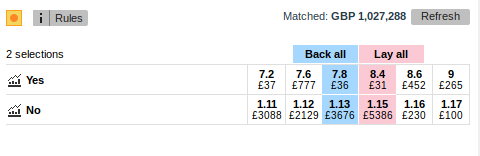
\includegraphics[width=0.9\textwidth]{Brexit_deal_betfair.png}
\caption{Odds on Betfair, 2019-02-28}
\label{fig:odds:betfair}
\end{center}
\end{figure}
\begin{figure}[htb]
\begin{center}
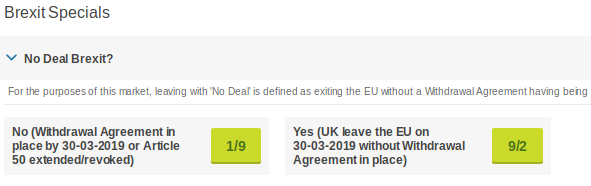
\includegraphics[width=0.9\textwidth]{Brexit_deal_paddy_power.png}
\caption{Odds on Paddy power, 2019-02-28}
\label{fig:odds:paddypower}
\end{center}
\end{figure}

What does all this mean? Is there an arbitrage opportunity?
We will come back to these two, first we need to understand how these odds work.


\section{Different types of odds}

There are various ways of expressing odds, with a good summery given on the Wikipedia articles on
odds\footnote{\url{https://en.wikipedia.org/wiki/Odds}}
and
fixed-odds betting.\footnote{\url{https://en.wikipedia.org/wiki/Fixed-odds_betting}}.
The only type of odds important to us are \emph{fractional odds} and \emph{decimal odds}.


\subsection{Fractional odds}
Fractional odds are also known as British odds, UK odds (or in the UK, traditional odds).
They may look weird, but are the easiest type of odds to use when gambling with your mates.
Consider this.
You say ``I bet we will leave the EU without a deal'' and I say ``OK, I'll give you 9 to 2''.
You want to bet on a no deal.
Here is another description of the bet we are considering:
\begin{align*}
\text{no}&/\text{yes}  \\
\text{deal}&/\text{no deal}  \\
9 &/ 2
\end{align*}
The wording is confusing, and that's usually what you need to be careful with.
In this scenario, betting on ``yes'' means you are backing ``no deal brexit''.
This simply means you put down 2, I put down 9, and winner takes all.
The help section on betting sites usually explain this as ``for every 2 you wager you can win 9'' but that doesn't help much.
The important thing to know is that these odds became popular because they are so useful when betting among friends.\footnote{something that is illegal in most countries, outside of the UK}
Later, professional bookmakers made the process more formal, and they usually sit on the ``left'' side of the equation given above.
They kept the familiar odds, even though it might not be the best way to think about odds when bookmaking. Hence the appearance of decimal odds, which we will consider in the next section.
With fractional odds, the thing you want to bet on should always go in the denominator.

First of all, is this a good bet? Let's look at the implied probabilities, since this is the most intuitive way to think about betting.
The expected value of a bet, in general, is:
\begin{align*}
E(Profit) &=
Winnings \times P(Win) +
Losses   \times P(Loss)
\end{align*}
For our bet on a no deal, let $p$ be the implied probability, then the expected profit is
\begin{align*}
E(Profit)
&=
(9)    \times P(Win) +
(-2)   \times P(Loss) \\
&= (9)    p  + (-2)  (1-p) \\
&= -2 + (9 + 2)p   \\
p &= \frac{2}{9 + 2}   \\
  &= \frac{2}{11}
\end{align*}
which comes to about 18\%.
What if you thought that 18\% seemed low, since you believed it to be higher. Should you take this bet?
We will get to that shortly.
First, let's turn the implied probability into a more general result.
Throughout this document we will use the following notation:
\begin{itemize}
 \item Let $s$ be the amount you stake (your potential losses)
 \item Let $w$ be your potential winnings (the amount your friend or the house stakes)
\end{itemize}
For a bet where I stake $s$ with the chance to win $w$,
\begin{align*}
\text{deal}&/\text{no deal}  \\
w &/ s  \\
\end{align*}
Let $p$ be the implied probability of winning the bet if the gamble is fair, then
\begin{align*}
E(Profit)
&=
(w)    \times P(Win) +
(-s)   \times P(Loss)  \\
&=
wp +
(-s)(1-p)  \\
&= -s + (s + w)p  \nonumber \\
\end{align*}
For a fair gamble, the expected profit must be zero,
\begin{align}
0
&= -s + (s + w)p  \nonumber \\
p &= \frac{s}{s + w} \label{eq:implied_prob}
\end{align}
and we will use this later to simplify things greatly.
But first, lets look at decimal odds.

\subsection{Decimal odds}
Decimal odds are also known as European odds, digital odds or continental odds.
They can loosely be thought of as ``return on investment,'' or ``return on stake''.
If we want to bet on ``yes'' (yes, there will be a no deal Brexit), we have to \emph{back} it.
\begin{itemize}
 \item When you \emph{back} something, you bet \emph{on} it.
 \item When you \emph{lay} something, you bet \emph{against} it.
\end{itemize}
Betfair provides a market,\footnote{It also provides a vanilla betting site, but the market is much more interesting.} which allows you to sit on both sides of the bet, meaning you get to be the bookmaker as well, if you so desire (this is when you ``lay'').
In figure \ref{fig:odds:betfair}, we see that we can back it at odds of 7.8
This means that, if we bet 1, we will get back 7.8 in total (including the stake of 1).
The definition of decimal odds, using our stake/winnings notation, is
\begin{align*}
 \text{Decimal odds} &=
\frac{s + w}{s}
\text{.}
\end{align*}
Note that this is the reciprocal of \eqref{eq:implied_prob}, making it easy to calculate the implied probability from the decimal odds.
This is one of the reasons for its popularity, another being that it is easier to see the market spread using decimal odds than fractional odds.
Figure \ref{fig:odds:betfair} is an example of this.

\subsection{Conversions}

To recap, if we have a stake $s$ with a winnings $w$, we can display it as either fractional or decimal
\begin{description}
 \item[Fractional] $w/s$
 \item[Decimal]    $\displaystyle \frac{s + w}{s}$
\end{description}
and the fractional odds will usually be displayed using the two smallest integers possible.
Remember: with fractional odds, the thing you want to bet on---the thing you want to back---is on the right side of the fraction, in the denominator.
The above shows that it is trivial to convert from fractional to decimal odds.

To convert from decimal to fractional is not that difficult, the only thing is that we have to choose a ``base'', or the value of $s$.
The easiest to use is a base of 1
Consider, for example, decimal odds of 7.8,
\begin{align*}
 7.8 &=  1 + 6.8 \\
     &= \frac{1 + 6.8}{1}
     \text{,}
\end{align*}
which means decimal odds of 7.8 are equivalent to fractional odds of $6.8/1$, or $34/5$.
Now we can convert both ways; between decimal and fractional and back, but things are still pretty confusing.
I will present a unifying theory below, but first, here is a table of decimal odds, implied probabilities, and fractional odds, using various bases.
% latex table generated in R 3.4.4 by xtable 1.8-3 package
% Wed Mar  6 07:11:44 2019
\begin{longtable}{rrrlll}
  \hline
Decimal & $p$ & Hong Kong & Fractional & Fractional/1 & Fractional sum 100 \\ 
  \hline
1.05 & 0.95 & 0.05 & 1/20 & 0.05/1 &  4.76 / 95.24 \\ 
  1.20 & 0.83 & 0.20 & 1/5 & 0.2/1 & 16.67 / 83.33 \\ 
  1.30 & 0.77 & 0.30 & 3/10 & 0.3/1 & 23.08 / 76.92 \\ 
  1.50 & 0.67 & 0.50 & 1/2 & 0.5/1 & 33.33 / 66.67 \\ 
  2.00 & 0.50 & 1.00 & 1 & 1/1 & 50.00 / 50.00 \\ 
  2.50 & 0.40 & 1.50 & 3/2 & 1.5/1 & 60.00 / 40.00 \\ 
  3.00 & 0.33 & 2.00 & 2 & 2/1 & 66.67 / 33.33 \\ 
  3.50 & 0.29 & 2.50 & 5/2 & 2.5/1 & 71.43 / 28.57 \\ 
  4.00 & 0.25 & 3.00 & 3 & 3/1 & 75.00 / 25.00 \\ 
  4.50 & 0.22 & 3.50 & 7/2 & 3.5/1 & 77.78 / 22.22 \\ 
  5.00 & 0.20 & 4.00 & 4 & 4/1 & 80.00 / 20.00 \\ 
  6.00 & 0.17 & 5.00 & 5 & 5/1 & 83.33 / 16.67 \\ 
  7.00 & 0.14 & 6.00 & 6 & 6/1 & 85.71 / 14.29 \\ 
  10.00 & 0.10 & 9.00 & 9 & 9/1 & 90.00 / 10.00 \\ 
   \hline
\hline
\end{longtable}

You may notice the most intuitive way to think about already, by looking at the $p$ column, and the column with ``Fractional sum 100''.
I'll explain it below.
A longer, more complete table is given in the appendix.


\subsection{A mnemonic}
To make odds interesting, we need a way to rapidly convert between the different types that is also easy to digest.
We need to be able to look at a set of odds and immediately spot the good deals or arbitrage opportunities.
I have made a three point ``mnemonic'' to make odds easier:


\begin{enumerate}
 \item Probability is Price.
 Remember it as $p$ is price, and always think in terms of the implied probabilities when you want to evaluate a deal. If the implied probability seems low, you need to buy. If it is high, you need to sell.
 \item Sum to hundred. Convert all odds into fractional that add to 1 (or 100).
 \item Back is Buy and Lay is Sell
\end{enumerate}

The first point is what you will use to quickly evaluate a gamble to see whether it is a good deal, and the second point will allow you to do it.
Converting odds to a fraction that sums to hundred makes it very easy to digest the odds, and what they mean.
This is also very easy to do. You calculate the implied probability of the odds and put it in the denominator, as a percentage.
Then you put $(1-p)$ in the nominator.

Say you believe that Brexit will happen with 30\% probability, and want to bet on it.
A friend agrees with the probability, but he wants to sit on the other side of the bet (he believes Brexit won't happen with 70\%.
What is the fair price for this gamble Bremain/Brexit?
The answer is simply:
\begin{align}
 \text{bremain}&/\text{brexit} \label{eq:brexitbet} \\
 70&/30 \nonumber \\
 7&/3  \nonumber
 \text{.}
\end{align}
So you put down 30, your friend puts down 70, and winner takes all.
This is the simplest way to do betting: put your money where you mouth is.
If you believe an event is 70\% percent likely to happen, put down £70.
This can also be extended to multiple outcome bets, like win/lose/draw.
As long as you ensure that all the numbers add to 100, it is easy to think about it.

\begin{proposition}
If an event will occur with probability $p$, the fair odds for a gamble that backs this event is
\begin{align}
(1-p)/p
\text{.}
\end{align}
\end{proposition}
\begin{proof}
For the gamble to be fair, we need the expected value to be zero:
\begin{align*}
E(Profit)
&=
(w)    \times P(Win) +
(-s)   \times P(Loss)  \\
&=
wp +
(-s)(1-p)
\text{.}
\end{align*}
If we let $w=(1-p)$ and $s=p$, this becomes
\begin{align*}
E(Profit)
&=
(1-p)p +
(-p)(1-p)
\end{align*}
\end{proof}



Let's look at this Brexit gamble again, but we'll expressed in decimal odds, which will show that it is not as intuitive as the fractional-sum-hundred odds.
The decimal equivalent of the bet in \eqref{eq:brexitbet} is
\begin{align*}
 \text{Odds for Brexit} \\
 \frac{70 + 30}{30} = 3.33333 \text{.}
\end{align*}
You will \emph{back} these odds, and your friend would \emph{lay} them, but it is not immediately clear how much you need to put down, and how much your friend needs to put down.
From your friend's perspective, it will look like this:
\begin{align*}
 \text{Odds for Bremain} \\
 \frac{70 + 30}{70} =
 1.428571
 \text{.}
\end{align*}
Again, it is not clear how much each of you should wager.

Simplicity is what made fractional odds so popular for informal, friendly betting.
Bookmaking adds complexity on it, since the bookmaker needs to sit between you and your friend, and needs to make a guaranteed profit.
For bookmakers, Decimal odds makes more sense, since the simplicity of fractional odds aren't of help to them (they will always sit on the ``left'' side of the odds, so they might as well just quote you your potential returns).
We will look at the mechanics of bookmaking below, and how you can identify and construct your own ``dutch book'', where a profit is guaranteed no matter the outcome.
The process for setting up profitable trades is similar.

\section{Guaranteed profit}
\subsection{Betfair vs Paddy Power}

The final element here is to spot arbitrage opportunities.
Let's consider the Betfair \emph{vs} Paddy power examples above.
First, we will convert them to fractional odds, that sum to 100.
For Betfair, we have from figure \ref{fig:odds:betfair} (ignoring the market depth):

\begin{center}
\begin{tabular}{ccc}
\hline
       &  Back     &   Lay    \\
Yes    &   7.8     &   8.4    \\
No     &   1.13    &   1.15   \\
\hline
\end{tabular}
\end{center}
Let's use our mnemonic and convert this into fractional odds that sum to 100, and replace back/lay with buy/sell.
Remember, $p = \frac{1}{\text{Decimal odds}}$.
\begin{center}
\begin{tabular}{ccc}
\hline
       &  Buy     &   Sell      \\
Yes    &   \odds{12.82}   &   \odds{11.90}    \\
No     &   \odds{88.49}   &   \odds{86.95}  \\
\hline
\end{tabular}
\end{center}
Take note, your price is the \emph{right} side of the fraction.
I also introduce a new notation that expresses the left side of the fraction in small font.
This is to highlight the important denominator on the right, but I still include the nominator, since we may want to use it for comparison.%
\footnote{
For instance, selling ``yes'' is the same as buying ``no''. In this example, we can sell yes at \odds{11.90},
or we can buy ``no'' at \odds{88.49}, which is like selling yes at 11.51.
We would rather sell as high as we can, so we prefer selling ``yes'' to buying ``no''.
We can quickly see this if the notation also includes the small numbers in the nominator.
}
Betfair is special, since we get to buy and sell. Buying yes is the same as selling no, and we need to check which price is the best (here, the fractional that adds to 100 helps again).

Now look at Paddy Power. Since this is not an exchange, we can only back (buy):
\begin{center}
\begin{tabular}{ccc}
\hline
       &  Back    \\
Yes    &   1/9   \\
No     &   9/2   \\
\hline
\end{tabular}
\end{center}
Using the mnemonic:
\begin{center}
\begin{tabular}{ccc}
\hline
       &  Buy           \\
Yes     &   \odds{18.18}   \\
No      &   \odds{90.00}   \\
\hline
\end{tabular}
\end{center}
\begin{itemize}
 \item We can buy ``Yes'' on Paddy Power for 18.18 and sell it on Betfair for 11.90 (or 11.51 if we buy No)
 \item We can buy ``No'' on Paddy Power for 90 and sell it on Betfair for 86.95
\end{itemize}
Both of these are bad deals. We don't want to buy high and sell low.
There is no arbitrage available here.\footnote{Big surprise.}
Also note that Betfair has better prices than Paddy Power in this instance,

\subsection{A bet with friends}

Pretend that you have a friend.
One who believes strongly in a no deal Brexit.
He thinks there is a 30\% probability that a no deal Brexit will happen (about 1 in 3 chance).
You tell him to put his money where his mouth is, and you agree to give him these odds (because you think it's more like 10\%).
He will bet on ``Yes'' by backing it, and you will lay it.
From your perspective:
\begin{center}
\begin{tabular}{ccc}
\hline
       &    Lay (sell)   \\
Yes    &  \odds{30.00}   \\
\hline
\end{tabular}
\end{center}
You are selling this bet to him, meaning
you are sitting on the left side so you stake 70, but the ``price'' you are selling at is 30.
This is where it can get confusing, but working through a few examples will give you clarity.
Now, remember that the odds on Betfair were:
\begin{center}
\begin{tabular}{ccc}
\hline
       &  Buy     &   Sell      \\
Yes    &   \odds{12.82}   &   \odds{11.90}    \\
No     &   \odds{88.49}   &   \odds{86.95}  \\
\hline
\end{tabular}
\end{center}
You can buy the bet you sold to your friend for 30.00 at 12.82!
Here is how to ensure a profit. The odds that sum to 100 makes it really easy.

Lay 70 in the bet with your friend, and back 12.82 on betfair.
Your situation now looks like this:
\begin{center}
\begin{tabular}{ccc}
\hline
                   &     Yes           &  \\
Bet with friend    &   (70)/30         &  \\
Betfair            &   87.18/(12.82)   &  \\
\hline
\end{tabular}
\end{center}
The numbers in brackets are what you put down: it is your liability.
To enter this ``trade'' cost you 70 + 12.82 = 82.82.
This is an investment, you'll have to leave this money in the pot until the outcome is reached.
On the day of the event, yes or no will happen, and your profits are:
\begin{center}
\begin{tabular}{cc|c|c}
\hline
                  &  Profit if Yes &                   & Profit if No  \\
                  &                &      Yes          &               \\
Bet with friend   &  -70           &   (70)/30         &  30           \\
Betfair           &   87.18        &   87.18/(12.82)   &  -12.82       \\
\hline
Total             &   17.18        &                   &  17.18       \\
\hline
\end{tabular}
\end{center}

Whatever happens, you win 17.18. Your return is
\begin{align*}
 \frac{82.82 + 17.18}{82.82}
 &=
 \frac{100}{82.82}
\end{align*}
and you have to adjust it for the period for which your money was locked up if you want the annual return.

Basically, if you always keep in mind what the Betfair probabilities are about big events, you can almost always do something like this, because the Betfair odds have a very tight spread. whatever number your friend quotes is unlikely to be the same as the market, so you can often hedge yourself. 
Remember, you'll usually sell to them, so if their estimate of the probability of an even is higher than Betfair, you can make money!


\subsection{Market moves in your favour}
Consider, again, the odds in figure \ref{fig:odds:betfair}.
\begin{center}
\begin{tabular}{ccc}
\hline
       &  Buy     &   Sell      \\
Yes    &   \oddsptodecimal{12.82}   &   \oddsptodecimal{11.90}    \\
No     &   \oddsptodecimal{88.49}   &   \oddsptodecimal{86.95}  \\
\hline
\end{tabular}
\end{center}
written using our mnemonic:
\begin{center}
\begin{tabular}{ccc}
\hline
       &  Buy     &   Sell      \\
Yes    &   \odds{12.82}   &   \odds{11.90}    \\
No     &   \odds{88.49}   &   \odds{86.95}  \\
\hline
\end{tabular}
\end{center}
Suppose you know something the market does not, making you believe that ``yes'', a no deal, will happen with probability 35\%.
The market is currently offering you this probability \emph{cheaper}, so you decide to buy it for 12.82, spending £12.82.


One week later, you see the following on Betfair:
\begin{center}
\begin{tabular}{ccc}
\hline
       &  Buy     &   Sell      \\
Yes    &   \oddsptodecimal{22.82}   &   \oddsptodecimal{21.90}    \\
No     &   \oddsptodecimal{78.49}   &   \oddsptodecimal{76.95}  \\
\hline
\end{tabular}
\end{center}
Is this good news? Let's check using our mnemonic:
\begin{center}
\begin{tabular}{ccc}
\hline
       &  Buy     &   Sell      \\
Yes    &   \odds{22.82}   &   \odds{21.90}    \\
No     &   \odds{78.49}   &   \odds{76.95}  \\
\hline
\end{tabular}
\end{center}
The probability has moved closer to what you believe it to be, and you decide to cash out now, rather than pushing your luck.
Betfair has an option called ``cash out'', which will place the right bet to allow you to realise your profit.
The right bet is to sell ``yes'' for £78.10, meaning we will have the following positions:
\begin{center}
\begin{tabular}{lc|c|c}
\hline
                         &  Profit if Yes &                   & Profit if No \\
                         &                &   No/Yes          &              \\
Betfair                  &   87.18        &   87.18/(12.82)   &  -12.82      \\
Betfair (one week later) &  -78.10        &   (78.10)/21.90   &   21.90      \\ \hline
Total                    &    9.08        &                   &   9.08       \\
\hline
\end{tabular}
\end{center}
You spent 12.82 + 78.10 on the two bets, and your profit was 9.08, giving you a return of $100/90.92$.
I don't actually know whether Betfair requires you to put down the £78.10 needed to cash out, I will need to investigate.

Keep in mind, however, that in this situation the market moved in your favour.
This won't always happen. It could very well be the case that the market stays ``wrong'' all the way through, and then ``No'' actually happens.
In this case, you would lose money, since you will never be able to cash out your bet at a better price.
It is also a philosophical question.
If the actual outcome in the end is ``No'', what was the \emph{true} probability of ``yes''?
This is something we can never truly determine.

\subsection{Bookmaking and the Dutch Book}

For the sake of completeness, I will also explain how bookmaking works.
Trading and bookmaking, while related, aren't similar.
When bookmakers make a book, they use something called ``over rounding''.
Consider the Brexit bet again.
The logic will generalise to bets with more than two outcomes, but it is best to stick with what we know for now.
Suppose the bookmaker has an accurate model, and thinks that ``yes'' will happen with probability 20\%.
We have already seen that the fair odds for yes would be \odds{20.00}.
If the bookmaker prices both bets fairly, have the following market (from the perspective of the customer):
\begin{center}
\begin{tabular}{ccc}
\hline
       &  Buy             \\
Yes    &   \odds{20.00}   \\
No     &   \odds{80.00}   \\
\hline
\end{tabular}
\end{center}
Let's say the bookmaker sells one of each of these bets above.
We have to change our table now, since the bookmaker has multiple bets.
The bookmaker sits on the ``left'' side of the bet, since they sell the bet.
\begin{center}
\begin{tabular}{lccc}
\hline
Outcome                  &   Odds              & Profit     & Total \\
 Yes                     &    (80.00)/20.00    & (80)  + 80 &  0    \\
 No                      &    (20.00)/80.00    & (20)  + 20 &  0    \\ \hline
\hline
\end{tabular}
\end{center}
In reality the bookmaker will now actually ``over round'' the book, so that the implied probabilities add up to more than 100\%. This is known as a dutch book:
\begin{center}
\begin{tabular}{ccc}
\hline
       &  Buy             \\
Yes    &   \odds{22.00}   \\
No     &   \odds{82.00}   \\
\hline
\end{tabular}
\end{center}
Note that, since the bookmaker believes the true odds to be 20\%, the price isn't fair.
The bookmaker is charging something akin to a market spread.
and then the outcomes will look like this.
\begin{center}
\begin{tabular}{lccc}
\hline
Outcome                  &   Odds              & Profit     & Total \\
 Yes                     &    (78.00)/22.00    & (78)  + 82 &  4    \\
 No                      &    (18.00)/82.00    & (18)  + 22 &  4    \\ \hline
\hline
\end{tabular}
\end{center}
This, however, assumes the bookmaker can balance the book, and sell one of each of the bets above. If they don't, the book will be unbalanced.
This is the risk that the bookmaker assumes, and the value they add to the economy is doing the work of matching all the bets.
If you want to bet on Brexit, you don't have to call all your friends and harass them, you just go the bookmaker and stake there.
The bookmaker will do the harassing for you, finding people to sit on the other side of your bet.

Look again at Paddy Power, and notice the overrounding:
\begin{center}
\begin{tabular}{ccc}
\hline
       &  Back    \\
Yes    &   1/9   \\
No     &   9/2   \\
\hline
\end{tabular}
\end{center}
Using the mnemonic:
\begin{center}
\begin{tabular}{ccc}
\hline
       &  Buy           \\
Yes     &   \odds{18.18}   \\
No      &   \odds{90.00}   \\
\hline
\end{tabular}
\end{center}
The implied probability for ``yes'' is 18.18\%, and the implied probability for ``no'' is 90\%.
This adds to more than 100\%.
For every £81.82 that the bookmaker stakes/matches, they will take in £100.



\clearpage
\appendix
\section{Conversion table}
% latex table generated in R 3.4.4 by xtable 1.8-3 package
% Wed Mar  6 07:11:44 2019
\begin{longtable}{rrrlll}
  \hline
Decimal & $p$ & Hong Kong & Fractional & Fractional/1 & Fractional sum 100 \\ 
  \hline
1.05 & 0.95 & 0.05 & 1/20 & 0.05/1 &  4.76 / 95.24 \\ 
  1.10 & 0.91 & 0.10 & 1/10 & 0.1/1 &  9.09 / 90.91 \\ 
  1.20 & 0.83 & 0.20 & 1/5 & 0.2/1 & 16.67 / 83.33 \\ 
  1.30 & 0.77 & 0.30 & 3/10 & 0.3/1 & 23.08 / 76.92 \\ 
  1.40 & 0.71 & 0.40 & 2/5 & 0.4/1 & 28.57 / 71.43 \\ 
  1.50 & 0.67 & 0.50 & 1/2 & 0.5/1 & 33.33 / 66.67 \\ 
  1.60 & 0.62 & 0.60 & 3/5 & 0.6/1 & 37.50 / 62.50 \\ 
  1.70 & 0.59 & 0.70 & 7/10 & 0.7/1 & 41.18 / 58.82 \\ 
  1.80 & 0.56 & 0.80 & 4/5 & 0.8/1 & 44.44 / 55.56 \\ 
  1.90 & 0.53 & 0.90 & 9/10 & 0.9/1 & 47.37 / 52.63 \\ 
  2.00 & 0.50 & 1.00 & 1 & 1/1 & 50.00 / 50.00 \\ 
  2.10 & 0.48 & 1.10 & 11/10 & 1.1/1 & 52.38 / 47.62 \\ 
  2.20 & 0.45 & 1.20 & 6/5 & 1.2/1 & 54.55 / 45.45 \\ 
  2.30 & 0.43 & 1.30 & 13/10 & 1.3/1 & 56.52 / 43.48 \\ 
  2.40 & 0.42 & 1.40 & 7/5 & 1.4/1 & 58.33 / 41.67 \\ 
  2.50 & 0.40 & 1.50 & 3/2 & 1.5/1 & 60.00 / 40.00 \\ 
  2.60 & 0.38 & 1.60 & 8/5 & 1.6/1 & 61.54 / 38.46 \\ 
  2.70 & 0.37 & 1.70 & 17/10 & 1.7/1 & 62.96 / 37.04 \\ 
  2.80 & 0.36 & 1.80 & 9/5 & 1.8/1 & 64.29 / 35.71 \\ 
  2.90 & 0.34 & 1.90 & 19/10 & 1.9/1 & 65.52 / 34.48 \\ 
  3.00 & 0.33 & 2.00 & 2 & 2/1 & 66.67 / 33.33 \\ 
  3.10 & 0.32 & 2.10 & 21/10 & 2.1/1 & 67.74 / 32.26 \\ 
  3.20 & 0.31 & 2.20 & 11/5 & 2.2/1 & 68.75 / 31.25 \\ 
  3.30 & 0.30 & 2.30 & 23/10 & 2.3/1 & 69.70 / 30.30 \\ 
  3.40 & 0.29 & 2.40 & 12/5 & 2.4/1 & 70.59 / 29.41 \\ 
  3.50 & 0.29 & 2.50 & 5/2 & 2.5/1 & 71.43 / 28.57 \\ 
  3.60 & 0.28 & 2.60 & 13/5 & 2.6/1 & 72.22 / 27.78 \\ 
  3.70 & 0.27 & 2.70 & 27/10 & 2.7/1 & 72.97 / 27.03 \\ 
  3.80 & 0.26 & 2.80 & 14/5 & 2.8/1 & 73.68 / 26.32 \\ 
  3.90 & 0.26 & 2.90 & 29/10 & 2.9/1 & 74.36 / 25.64 \\ 
  4.00 & 0.25 & 3.00 & 3 & 3/1 & 75.00 / 25.00 \\ 
  4.10 & 0.24 & 3.10 & 31/10 & 3.1/1 & 75.61 / 24.39 \\ 
  4.20 & 0.24 & 3.20 & 16/5 & 3.2/1 & 76.19 / 23.81 \\ 
  4.30 & 0.23 & 3.30 & 33/10 & 3.3/1 & 76.74 / 23.26 \\ 
  4.40 & 0.23 & 3.40 & 17/5 & 3.4/1 & 77.27 / 22.73 \\ 
  4.50 & 0.22 & 3.50 & 7/2 & 3.5/1 & 77.78 / 22.22 \\ 
  4.60 & 0.22 & 3.60 & 18/5 & 3.6/1 & 78.26 / 21.74 \\ 
  4.70 & 0.21 & 3.70 & 37/10 & 3.7/1 & 78.72 / 21.28 \\ 
  4.80 & 0.21 & 3.80 & 19/5 & 3.8/1 & 79.17 / 20.83 \\ 
  4.90 & 0.20 & 3.90 & 39/10 & 3.9/1 & 79.59 / 20.41 \\ 
  5.00 & 0.20 & 4.00 & 4 & 4/1 & 80.00 / 20.00 \\ 
  5.10 & 0.20 & 4.10 & 41/10 & 4.1/1 & 80.39 / 19.61 \\ 
  5.20 & 0.19 & 4.20 & 21/5 & 4.2/1 & 80.77 / 19.23 \\ 
  5.30 & 0.19 & 4.30 & 43/10 & 4.3/1 & 81.13 / 18.87 \\ 
  5.40 & 0.19 & 4.40 & 22/5 & 4.4/1 & 81.48 / 18.52 \\ 
  5.50 & 0.18 & 4.50 & 9/2 & 4.5/1 & 81.82 / 18.18 \\ 
  5.60 & 0.18 & 4.60 & 23/5 & 4.6/1 & 82.14 / 17.86 \\ 
  5.70 & 0.18 & 4.70 & 47/10 & 4.7/1 & 82.46 / 17.54 \\ 
  5.80 & 0.17 & 4.80 & 24/5 & 4.8/1 & 82.76 / 17.24 \\ 
  5.90 & 0.17 & 4.90 & 49/10 & 4.9/1 & 83.05 / 16.95 \\ 
  6.00 & 0.17 & 5.00 & 5 & 5/1 & 83.33 / 16.67 \\ 
  6.10 & 0.16 & 5.10 & 51/10 & 5.1/1 & 83.61 / 16.39 \\ 
  6.20 & 0.16 & 5.20 & 26/5 & 5.2/1 & 83.87 / 16.13 \\ 
  6.30 & 0.16 & 5.30 & 53/10 & 5.3/1 & 84.13 / 15.87 \\ 
  6.40 & 0.16 & 5.40 & 27/5 & 5.4/1 & 84.38 / 15.62 \\ 
  6.50 & 0.15 & 5.50 & 11/2 & 5.5/1 & 84.62 / 15.38 \\ 
  6.60 & 0.15 & 5.60 & 28/5 & 5.6/1 & 84.85 / 15.15 \\ 
  6.70 & 0.15 & 5.70 & 57/10 & 5.7/1 & 85.07 / 14.93 \\ 
  6.80 & 0.15 & 5.80 & 29/5 & 5.8/1 & 85.29 / 14.71 \\ 
  6.90 & 0.14 & 5.90 & 59/10 & 5.9/1 & 85.51 / 14.49 \\ 
  7.00 & 0.14 & 6.00 & 6 & 6/1 & 85.71 / 14.29 \\ 
  7.10 & 0.14 & 6.10 & 61/10 & 6.1/1 & 85.92 / 14.08 \\ 
  7.20 & 0.14 & 6.20 & 31/5 & 6.2/1 & 86.11 / 13.89 \\ 
  7.30 & 0.14 & 6.30 & 63/10 & 6.3/1 & 86.30 / 13.70 \\ 
  7.40 & 0.14 & 6.40 & 32/5 & 6.4/1 & 86.49 / 13.51 \\ 
  7.50 & 0.13 & 6.50 & 13/2 & 6.5/1 & 86.67 / 13.33 \\ 
  7.60 & 0.13 & 6.60 & 33/5 & 6.6/1 & 86.84 / 13.16 \\ 
  7.70 & 0.13 & 6.70 & 67/10 & 6.7/1 & 87.01 / 12.99 \\ 
  7.80 & 0.13 & 6.80 & 34/5 & 6.8/1 & 87.18 / 12.82 \\ 
  7.90 & 0.13 & 6.90 & 69/10 & 6.9/1 & 87.34 / 12.66 \\ 
  8.00 & 0.12 & 7.00 & 7 & 7/1 & 87.50 / 12.50 \\ 
  8.10 & 0.12 & 7.10 & 71/10 & 7.1/1 & 87.65 / 12.35 \\ 
  8.20 & 0.12 & 7.20 & 36/5 & 7.2/1 & 87.80 / 12.20 \\ 
  8.30 & 0.12 & 7.30 & 73/10 & 7.3/1 & 87.95 / 12.05 \\ 
  8.40 & 0.12 & 7.40 & 37/5 & 7.4/1 & 88.10 / 11.90 \\ 
  8.50 & 0.12 & 7.50 & 15/2 & 7.5/1 & 88.24 / 11.76 \\ 
  8.60 & 0.12 & 7.60 & 38/5 & 7.6/1 & 88.37 / 11.63 \\ 
  8.70 & 0.11 & 7.70 & 77/10 & 7.7/1 & 88.51 / 11.49 \\ 
  8.80 & 0.11 & 7.80 & 39/5 & 7.8/1 & 88.64 / 11.36 \\ 
  8.90 & 0.11 & 7.90 & 79/10 & 7.9/1 & 88.76 / 11.24 \\ 
  9.00 & 0.11 & 8.00 & 8 & 8/1 & 88.89 / 11.11 \\ 
  9.10 & 0.11 & 8.10 & 81/10 & 8.1/1 & 89.01 / 10.99 \\ 
  9.20 & 0.11 & 8.20 & 41/5 & 8.2/1 & 89.13 / 10.87 \\ 
  9.30 & 0.11 & 8.30 & 83/10 & 8.3/1 & 89.25 / 10.75 \\ 
  9.40 & 0.11 & 8.40 & 42/5 & 8.4/1 & 89.36 / 10.64 \\ 
  9.50 & 0.11 & 8.50 & 17/2 & 8.5/1 & 89.47 / 10.53 \\ 
  9.60 & 0.10 & 8.60 & 43/5 & 8.6/1 & 89.58 / 10.42 \\ 
  9.70 & 0.10 & 8.70 & 87/10 & 8.7/1 & 89.69 / 10.31 \\ 
  9.80 & 0.10 & 8.80 & 44/5 & 8.8/1 & 89.80 / 10.20 \\ 
  9.90 & 0.10 & 8.90 & 89/10 & 8.9/1 & 89.90 / 10.10 \\ 
  10.00 & 0.10 & 9.00 & 9 & 9/1 & 90.00 / 10.00 \\ 
   \hline
\hline
\end{longtable}



\end{document}
